\documentclass{article} % For LaTeX2e
\usepackage{nips12submit_e,times}
%\documentstyle[nips12submit_09,times,art10]{article} % For LaTeX 2.09

\usepackage{amsmath}
\usepackage{graphicx}
\usepackage{url}

\renewcommand{\arraystretch}{1.5}
\DeclareMathOperator*{\argmax}{arg\,max}


\title{Multiple Representations, Problem-Solving Behavior and Educational Outcomes}


\author{
Helga Caballero \\
School of Public and International Affairs \\
University of Pittsburgh\\
Pittsburgh, PA 15260 \\
\texttt{hec33@pitt.edu} \\
\And
Ryan Carlson \\
Language Technologies Insitute \\
Carnegie-Mellon University \\
Pittsburgh, PA 15213 \\
\texttt{rcarlson@cs.cmu.edu} \\
\And
Konstantin Genin \\
Department of Philosophy \\
Carnegie-Mellon University \\
Pittsburgh, PA 15213 \\
\texttt{kgenin@andrew.cmu.edu} \\
}


% The \author macro works with any number of authors. There are two commands
% used to separate the names and addresses of multiple authors: \And and \AND.
%
% Using \And between authors leaves it to \LaTeX{} to determine where to break
% the lines. Using \AND forces a linebreak at that point. So, if \LaTeX{}
% puts 3 of 4 authors names on the first line, and the last on the second
% line, try using \AND instead of \And before the third author name.

\newcommand{\fix}{\marginpar{FIX}}
\newcommand{\new}{\marginpar{NEW}}

%\nipsfinalcopy % Uncomment for camera-ready version

\begin{document}



\maketitle


\begin{abstract}
We analyze log-data generated by an experiment with an intelligent tutoring system for fractions. The experiment was performed to compare the educational outcomes for students presented with single and multiple graphical representations. We extract features characterizing problem-solving behavior and its evolution over time. We use latent class analysis to cluster the students by their problem-solving behaviors, using extracted features as proxies. We then explore how these behaviors interact with the mode of representation and post-test outcomes. We find that while experimental condition and outcomes are unconditionally dependent, latent class membership screens off experimental condition from outcome for all but one class. We examine the properties of this class and their implications for the design of tutoring systems.
\end{abstract}

\section{Introduction}

Multiple graphical representations are used extensively in middle-school fraction instructions.  Fractions are alternately presented as pie and rectangle graphs, number lines and discrete sets of objects. The educational psychology literature suggests that multiple-representations support learning in a variety of ways, though the experimental results are not univocal [1]. Intelligent Tutoring Systems (ITS) are uniquely suited for conducting experiments on the effect of multiple representations on learning outcomes. ITSs capture a significant amount of log data on how students interact with the tutoring system -- suggesting that machine learning methods could effectively discern the effectiveness of MGRs and the factors mediating their success. 

Classroom studies conducted on middle-school students working with ITSs found that multiple representations, in conjunction with self-explanation prompts, contribute to better learning outcomes [2]. Subsequent studies examining error-rate, hint-use and time-spent in ITS logs failed to identify variables that mediate the effectiveness of multiple representations [3]. The mechanisms by which multiple representations improve learning outcomes remain poorly understood.

We conjecture that previous efforts to identify mediating factors were frustrated by heterogeneity in the problem-solving habits and behaviors of the student population under investigation. Using a Latent Class Model, we cluster students by their patterns of interaction with the tutor and examine how multiple representations affect post-test outcomes in the resulting sub-populations. Confirming previous results, we find dependence between experimental condition and post-test outcome. Furthermore, we establish independence between experimental condition and latent class membership. Most interestingly, we discover conditional independence between experimental condition and outcome, conditional on latent class membership for all but one sub-population of students.

\section{Experiment}
In the Spring of 2010, Scheines and Rau conducted an experiment wherein 290 $4^{th}$ and $5^{th}$ grade students worked with an interactive Fractions Tutor for about 5 hours of their mathematics instruction. Students were randomly assigned to one of five experimental conditions corresponding to different frequencies with which they would be presented with a new fraction representation. Students in the `Single' representation condition worked exclusively with either a number line, a circle or a rectangle exclusively. Students in the `Fully Interleaved' condition would see a different representation with every new problem. Students in the intermediate conditions would go longer before they were presented with a different representation.   
\begin{figure}[htbp]
\centering
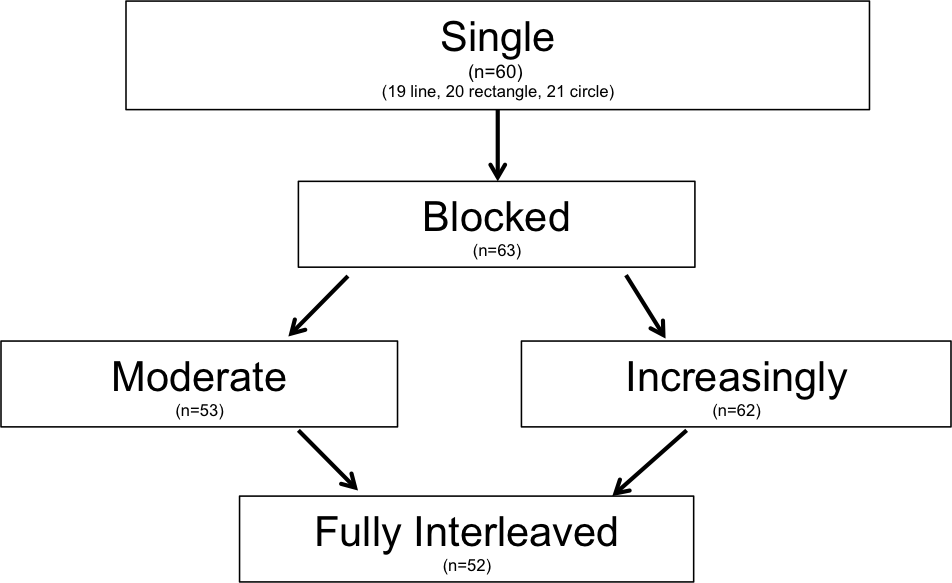
\includegraphics[scale=.4]{conditionGraph.png}\\
\caption{A partial ordering of experimental conditions by the frequency with which a new representation is presented. }
\label{fig:condition-graph}
\end{figure}

Students interacted with the representations by dragging-and-dropping sections of the representation, using buttons to change the number of sections and by clicking on sections to highlight them. Students received a pre-test on the day before they began working with the tutor and an immediate post-test on the day after they finished. Students also took a delayed post-test about a week after the first. Previous investigation found that students in the multiple representation conditions significantly outperformed students in the single representation condition [3]. 

\section{Method}
Our analysis proceeds in three stages. Extracting features characterizing error and hint-seeking behavior, we transform the longitudinal log data into a cross-sectional form, with one observation per student. We then run Latent Class Analysis to identify sub-populations of students, using AIC and BIC to select the number of latent classes. 

Once we have clustered our students, we investigate the interaction between the latent classes and their experimental conditions. We construct a contingency table binning the experimental conditions into the clusters estimated by the latent class model. We then run a $\mathcal{X}^2$ test, with a null hypothesis of independence between experimental condition and latent class, arriving at an exact $p$-level at which we can reject independence. $\mathcal{X}^2$ tests are also run to investigate dependence between latent class and post-test outcome and the conditional dependence of outcome and experimental condition, given latent class membership.

\subsection{Extracting Features}
The Cognitive Tutor captures a detailed log of the student's interactions with the tutor. It stores a time series of correct and incorrect answers, hint requests, interface selections and durations between interactions. Previous analysis (Scheines, Rau, 2012) extracted the average number of errors made per step, the average number of hints requested per step, and the average time spent per step from the log data. We include the average number of hints requested ($hints\_req$) and number of errors ($num\_errors$) made per problem by each student. We also extract the average number of bottom-out hints ($NumBOH$) per student per problem -- this is the average number of times a student exhausts the available hints in a given problem. We also note that it is not always the average of these features that best characterizes a student. For example, examination of the distribution of hints requested per step across experimental condition, shows a telling picture. 
\begin{figure}[htbp]
\centering
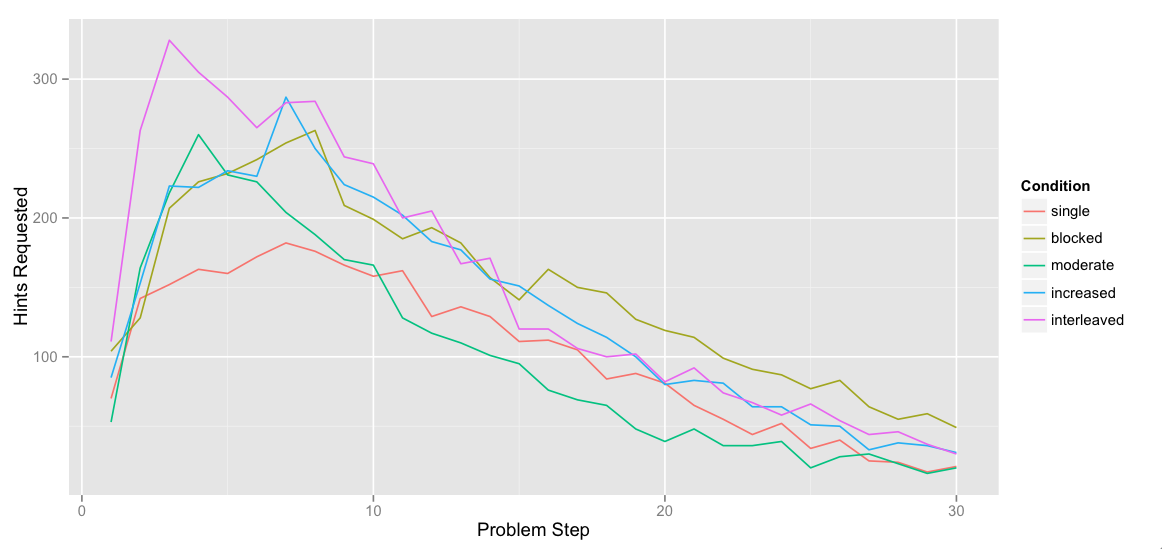
\includegraphics[scale=.35]{hintsByCondition.png}\\
\caption{The $x$-axis represents the $n_{th}$ interaction with the tutor across all problems. The $y$-axis is the total number of hints requested at the $n_{th}$ step.  }
\label{fig:condition-graph}
\end{figure}

Note that students who received only one representation start out requesting the fewest hints, but students in the moderate condition eventually need fewer. Such considerations motivated our interest in the temporal distribution of hint behavior at the student level. We fit geometric distributions to the number of steps taken before the first hint request ($firstHintGeom$) and to the number of errors before the first hint ($stubbornGeom$). The estimated parameter is used to characterize the student�s hint-seeking propensity in general and hint-seeking propensity when faced with adversity. For example, students in the first quintile of $stubbornGeom$ seek help soon after making a mistake, whereas students in the fifth quintile don�t change their hint-seeking behavior even after making a large number of errors. Students in the first quintile of $firstHintGeom$ are likely to request hints early in a problem, whereas students in the fifth quintile are unlikely to request hints at any point.
\begin{table}[htbp]
\caption{Summary Statistics for Variables Used in Clustering}
\begin{center}
\begin{tabular}{| c || c | c | c | c | c | c | c | c | c | c |}
\hline
&mean& sd&median&min&max&20\%&40\%&60\%&	80\%&100\%\\ \hline \hline
hints\_req&0.78&1.27&0.34&0&11.22&0.06&0.19&0.5&1.31&11.22\\ \hline
num\_errors&2.21&1.27&1.92&0.34&8.39&1.15&1.7&2.18&3.19&8.39\\ \hline 
firstHintGeom&0.35&0.27&0.27&0.04&1&0.13&0.2&0.33&0.57&1\\ \hline
stubbornGeom&0.36&0.21&0.31&0.07&1&0.19&0.27&0.38&0.47&1\\ \hline
NumBOH&0.04&0.08&0&0&0.62&0&0&0.01&0.05&0.63\\ \hline
 \end{tabular}
\end{center}
\label{default}
\end{table}

\subsection{Latent Class Analysis}
\label{sec:LCA}

Latent Class Analysis (LCA) is a modeling technique that determines subtypes based on multinomial distributions. Here, we use LCA to categorize students into \emph{latent classes} using features based on their behavior while interacting with Mathtutor. The model maps a set of categorical variables onto a set of inferred latent variables which are measured by observed variables. LCA is used widely in the behavioral, social, and educational sciences.

We note that the categorical nature of the model has the potential to add some noise, since we must select numeric cutoffs to transform our variables into nominals. However, categorical models can offer greater interpretability by allowing us to organize our data into a small set of variables, which forms the basis for categorizing students into a small set of meaningful homogenous groups. Furthermore, it is not unreasonable to suspect that our variables are in some sense ``truly'' categorical. 

The formal representation of LCA begins with $j = 1 \ldots J$ observed variables, where each such variable $j$ has a set of response variables $r_{j} = 1,\ldots,R_{j}$. Let some $y = (r_{1},\ldots,r_{j})$ be a response patterns with each response pattern $y$ is associated with some probability $P(Y = y)$ with \[ \sum P(Y = y) = 1. \]

Now, we need to consider the latent classes. Let $L$ be a latent variable with latent classes $c = 1,\ldots,C$. Furthermore, let $\gamma_{c}$ be the probability of membership in class $c$. Note that latent classes are exhaustive and mutually exclusive, so each student is a member of exactly one latent class. Formally,
\[ \sum_{c=1}^{C} \gamma_{c} = 1. \] 
We also need to define the item-response probability $\rho_{j,r_{j}|c}$, which is the probability of response $r_{j}$ to observed variable $j$, conditional on membership in latent class $c$. Note that 
\[ \sum_{r_{j}=1}^{R_{j}} \rho_{j,r_{j}|c} = 1 \] 
because each student provides exactly one response alternative to variable $j$. 

Now that we have defined key variables, we can define the probability of observing a particular response vector based on the $\gamma$'s and $\rho$'s:
\begin{align}
P(Y = y) = \sum_{c=1}^{C} \gamma_{c} \prod_{j=1}^{J} \prod_{r_{j}=1}^{R_{j}} \rho_{j,r_{j}|c}^{I(y_{j} = r_{j})}
\label{eqn:LCA-final}
\end{align}
where the indicator function $I(y_{j} = r_{j})$ equals 1 when the response variable $j = r_{j}$. The parameters $\gamma_{c}$ and $\rho_{j,r_{j}|c}$ are estimated by EM. Since EM is sensitive to starting probabilities, we pick the maximum likelihood over multiple (here, 25) runs. LCA is very similar to other EM-based algorithms. In fact, LCA is an application of multivariate mixture estimation using categorical variables with one additional assumption: a local independence assumption, meaning that the observed variables are independent of each other conditional on the latent variable. This is an assumption similar to the simplifying assumption made in Naive Bayes, in that without it Equation \ref{eqn:LCA-final} would need to be much more complicated. There is some work on relaxing this independence assumption [5]. To run latent class analysis, we used \texttt{poLCA}, a freely available R package\footnote{\url{http://userwww.service.emory.edu/~dlinzer/poLCA/}}.


Note that unlike some common clustering algorithms (e.g., k-means), LCA produces ``fuzzy'' clusters--probability distributions over features for each class. To cluster students we just identify their most likely class:
\begin{align}
\argmax_{c} P(Y = y \;|\; L = c) = \argmax_{c} \gamma_{c} \prod_{j=1}^{J} \prod_{r_{j}=1}^{R_{j}} \rho_{j,r_{j}|c}^{I(y_{j} = r_{j})}
\label{eqn:LCA-argmax}
\end{align}

We still need to fix $C$, the number of latent classes. We use two complexity-penalized log-likelihood scores as measures of fit to select an appropriate $C$: Akaike information criterion (AIC) and Bayesian information criterion (BIC). Plotting these statistics as we increment the number of latent classes, we look for a ``knee'' where both statistics either bottom-out or level off to identify the optimal value of $C$.

\section{Results}

We explore the relationships between latent classes, outcome measures, and experimental condition (i.e., representation of fractions) by first identifying and describing the latent classes and then analyzing independence relationships between these variables.

\subsection{Choosing the Number of Latent Classes}

As we described in Section \ref{sec:LCA}, we calculate complexity-penalized log-likelihood scores (AIC and BIC) as we increase the number of latent classes in the model and look for the ``knee'' of both statistics to agree. Figure \ref{fig:lca-test-statistics} shows this process. Note that we chose to model four latent classes because BIC bottoms out and AIC levels off at that point.

\begin{figure}[htbp]
\centering
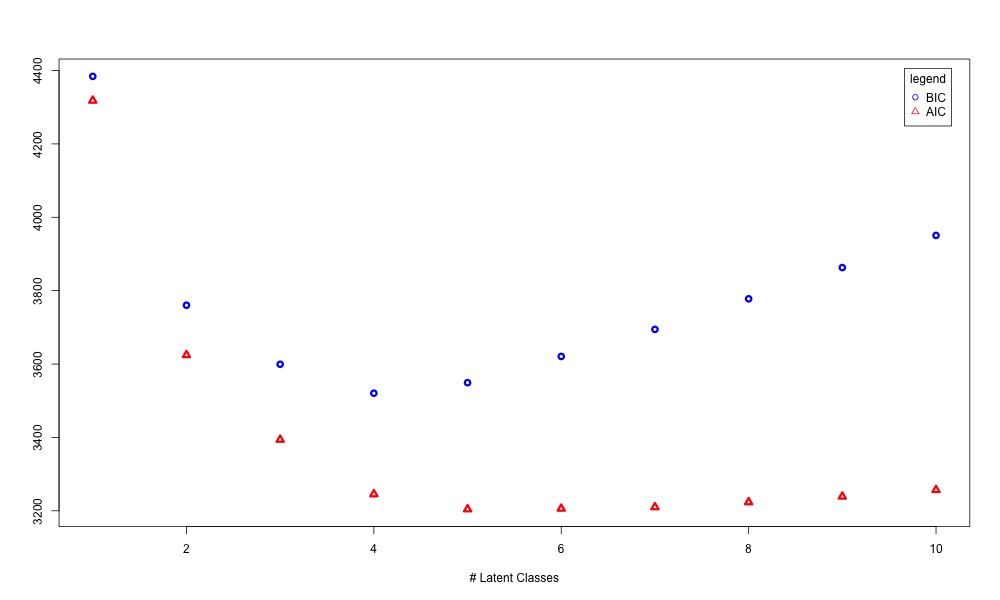
\includegraphics[scale=0.4]{lca-stats-plot.png}
\caption{AIC and BIC over increasing number of latent classes. BIC bottoms out and AIC levels off at four classes, so we conclude that four latent classes best fits the data.}
\label{fig:lca-test-statistics}
\end{figure}

\subsection{Exploring the Latent Classes}

After identifying the right number of latent classes to use, we can extract probabilities for each student. That is, given a latent class, we know the probability distribution over each feature, so we can use Equation \ref{eqn:LCA-argmax} to identify the most likely class for each student.

The feature distributions over each class are represented graphically in Figure \ref{fig:lca-class-viz}. Note that each feature is listed along the horizontal $x$-axis, the value each variable takes takes is along the front-to-back $y$-axis, and the probability that the feature takes that value is given along the vertical $z$-axis. For example, consider the \emph{hints\_req} feature (average hints requested per problem) in Class 1. In that class, with high probability, students requested many hints (i.e., the highest categorical value for hints) per problem on average. As another example, students in Class 3 are more likely to make a moderate number os errors, though other error levels also occur with nontrivial probabilities. Note that lower values of \emph{hintsGeom} and \emph{stubbornGeom} indicate a steep geometric slope, which translates to responsive behavior with the interface.

So, we are interested in summarizing characteristic student behavior in each class. We call students in Class 1 ``Interactive'' because these students need help (they make a lot of errors), request many hints, and exhibit responsive behaviors. Class 2 contain students who are ``Stubborn''--they don't ask for hints and don't change their hint-seeking behavior over time, and they are generally undifferentiated by the number of errors they make. Students in Class 3 are ``Moderate'' because they ask for a moderate number of hints, make a moderate number of errors, and are moderately responsive to the interface. Finally, in Class 4 students are ``Confident'' in that they don't ask for hints, but they also don't generally need hints (because they make very few errors).

\begin{figure}[htbp]
\centering
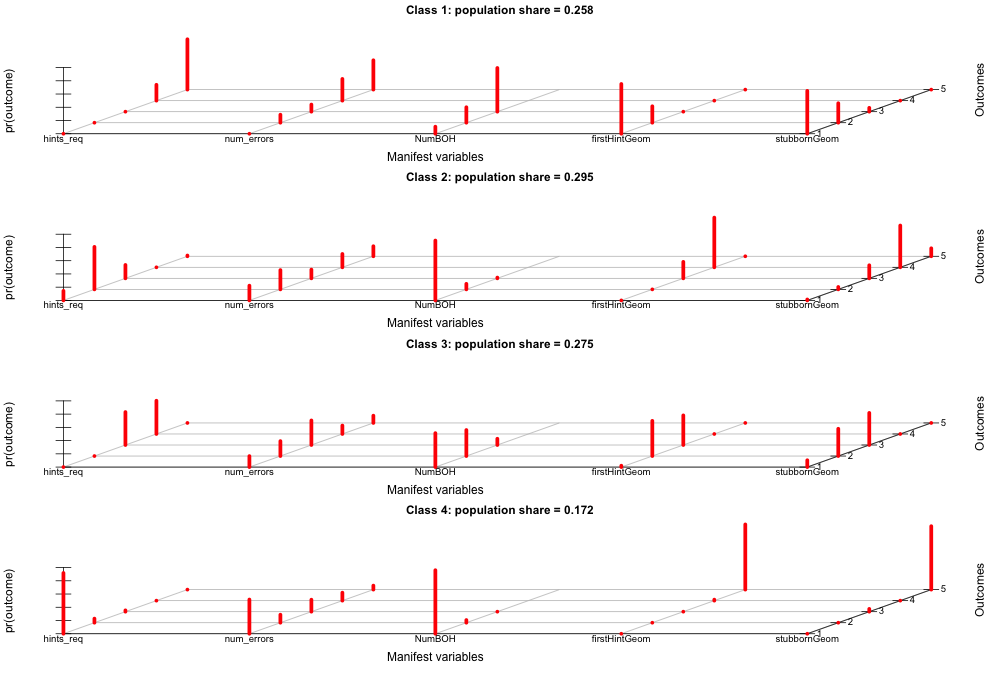
\includegraphics[scale=0.4]{lca-class-viz.png}
\caption{Visualization of feature distributions for each latent class. The left-to-right $x$-axis identifies each feature, the front-to-back $y$-axis identifies which value that feature takes, and the top-to-bottom $z$-axis describes the probability that the feature takes the value. Thus, given a feature and a class, the $z$-axis also describes the probability distribution over that feature in that class.}
\label{fig:lca-class-viz}
\end{figure}

\subsection{Condition and Cluster Membership}

Once clusters have been established, we will use Fisher's exact test to determine cluster dependence or independence from condition. 

\renewcommand{\arraystretch}{1}
\begin{table}[hbtp]
\caption{Condition by Tercile of Adjusted Delayed Post-Test Score (left) and Latent Class (right).}
 \begin{center}
\begin{tabular}{|c || c | c | c |}
\hline
&33\%&66\%&99\%\\ \hline \hline
  blocked  &   14& 29& 20 \\ \hline
  increased&   22& 20& 20 \\ \hline
  interleaved& 13& 21& 18 \\ \hline
  moderate &   18& 13& 22 \\ \hline
  single &      30& 13& 17 \\ \hline
 \end{tabular}
%\end{center}
\label{default}
%\end{table}
\quad
%\begin{table}[hbtp]
%\caption{Experimental Condition and Latent Class}
% \begin{center}
\begin{tabular}{|c || c | c | c | c |}
\hline
&LC1&LC2&LC3&LC4\\ \hline \hline
blocked&     25& 15& 10& 13\\ \hline
increased&   15& 16& 10& 21\\ \hline
interleaved& 10& 18&  7& 17\\ \hline
moderate&    13& 10& 12& 18\\ \hline
single&      20& 14& 11& 15\\ \hline
 \end{tabular}
 \end{center}
\hspace{32pt}$\mathcal{X}^2$ = 17.65, df = 8, p-value = 0.024\hspace{30pt}$\mathcal{X}^2$ = 12.85, df = 12, p-value = 0.38
\label{default}
\end{table}

\subsection{Cluster Membership and Outcome}

We will also run a similar analysis to analyze independence of cluster membership with respect to outcome.

\section{Conclusion}

Forthcoming.




%Papers to be submitted to NIPS 2012 must be prepared according to the
%instructions presented here. Papers may be only up to eight pages long,
%including figures. Since 2009 an additional ninth page \textit{containing only
%cited references} is allowed. Papers that exceed nine pages will not be
%reviewed, or in any other way considered for presentation at the conference.
%%This is a strict upper bound. 
%
%Please note that this year we have introduced automatic line number generation
%into the style file (for \LaTeXe and Word versions). This is to help reviewers
%refer to specific lines of the paper when they make their comments. Please do
%NOT refer to these line numbers in your paper as they will be removed from the
%style file for the final version of accepted papers.
%
%The margins in 2012 are the same as since 2007, which allow for $\approx 15\%$
%more words in the paper compared to earlier years. We are also again using 
%double-blind reviewing. Both of these require the use of new style files.
%
%Authors are required to use the NIPS \LaTeX{} style files obtainable at the
%NIPS website as indicated below. Please make sure you use the current files and
%not previous versions. Tweaking the style files may be grounds for rejection.
%
%%% \subsection{Double-blind reviewing}
%
%%% This year we are doing double-blind reviewing: the reviewers will not know 
%%% who the authors of the paper are. For submission, the NIPS style file will 
%%% automatically anonymize the author list at the beginning of the paper.
%
%%% Please write your paper in such a way to preserve anonymity. Refer to
%%% previous work by the author(s) in the third person, rather than first
%%% person. Do not provide Web links to supporting material at an identifiable
%%% web site.
%
%%%\subsection{Electronic submission}
%%%
%%% \textbf{THE SUBMISSION DEADLINE IS JUNE 1, 2012. SUBMISSIONS MUST BE LOGGED BY
%%% 23:00, JUNE 1, 2012, UNIVERSAL TIME}
%
%%% You must enter your submission in the electronic submission form available at
%%% the NIPS website listed above. You will be asked to enter paper title, name of
%%% all authors, keyword(s), and data about the contact
%%% author (name, full address, telephone, fax, and email). You will need to
%%% upload an electronic (postscript or pdf) version of your paper.
%
%%% You can upload more than one version of your paper, until the
%%% submission deadline. We strongly recommended uploading your paper in
%%% advance of the deadline, so you can avoid last-minute server congestion.
%%%
%%% Note that your submission is only valid if you get an e-mail
%%% confirmation from the server. If you do not get such an e-mail, please
%%% try uploading again. 
%
%
%\subsection{Retrieval of style files}
%
%The style files for NIPS and other conference information are available on the World Wide Web at
%\begin{center}
%   http://www.nips.cc/
%\end{center}
%The file \verb+nips2012.pdf+ contains these 
%instructions and illustrates the
%various formatting requirements your NIPS paper must satisfy. \LaTeX{}
%users can choose between two style files:
%\verb+nips11submit_09.sty+ (to be used with \LaTeX{} version 2.09) and
%\verb+nips11submit_e.sty+ (to be used with \LaTeX{}2e). The file
%\verb+nips2012.tex+ may be used as a ``shell'' for writing your paper. All you
%have to do is replace the author, title, abstract, and text of the paper with
%your own. The file
%\verb+nips2012.rtf+ is provided as a shell for MS Word users.
%
%The formatting instructions contained in these style files are summarized in
%sections \ref{gen_inst}, \ref{headings}, and \ref{others} below.
%
%%% \subsection{Keywords for paper submission}
%%% Your NIPS paper can be submitted with any of the following keywords (more than one keyword is possible for each paper):
%
%%% \begin{verbatim}
%%% Bioinformatics
%%% Biological Vision
%%% Brain Imaging and Brain Computer Interfacing
%%% Clustering
%%% Cognitive Science
%%% Control and Reinforcement Learning
%%% Dimensionality Reduction and Manifolds
%%% Feature Selection
%%% Gaussian Processes
%%% Graphical Models
%%% Hardware Technologies
%%% Kernels
%%% Learning Theory
%%% Machine Vision
%%% Margins and Boosting
%%% Neural Networks
%%% Neuroscience
%%% Other Algorithms and Architectures
%%% Other Applications
%%% Semi-supervised Learning
%%% Speech and Signal Processing
%%% Text and Language Applications
%
%%% \end{verbatim}
%
%\section{General formatting instructions}
%\label{gen_inst}
%
%The text must be confined within a rectangle 5.5~inches (33~picas) wide and
%9~inches (54~picas) long. The left margin is 1.5~inch (9~picas).
%Use 10~point type with a vertical spacing of 11~points. Times New Roman is the
%preferred typeface throughout. Paragraphs are separated by 1/2~line space,
%with no indentation.
%
%Paper title is 17~point, initial caps/lower case, bold, centered between
%2~horizontal rules. Top rule is 4~points thick and bottom rule is 1~point
%thick. Allow 1/4~inch space above and below title to rules. All pages should
%start at 1~inch (6~picas) from the top of the page.
%
%%The version of the paper submitted for review should have ``Anonymous Author(s)'' as the author of the paper.
%
%For the final version, authors' names are
%set in boldface, and each name is centered above the corresponding
%address. The lead author's name is to be listed first (left-most), and
%the co-authors' names (if different address) are set to follow. If
%there is only one co-author, list both author and co-author side by side.
%
%Please pay special attention to the instructions in section \ref{others}
%regarding figures, tables, acknowledgments, and references.
%
%\section{Headings: first level}
%\label{headings}
%
%First level headings are lower case (except for first word and proper nouns),
%flush left, bold and in point size 12. One line space before the first level
%heading and 1/2~line space after the first level heading.
%
%\subsection{Headings: second level}
%
%Second level headings are lower case (except for first word and proper nouns),
%flush left, bold and in point size 10. One line space before the second level
%heading and 1/2~line space after the second level heading.
%
%\subsubsection{Headings: third level}
%
%Third level headings are lower case (except for first word and proper nouns),
%flush left, bold and in point size 10. One line space before the third level
%heading and 1/2~line space after the third level heading.
%
%\section{Citations, figures, tables, references}
%\label{others}
%
%These instructions apply to everyone, regardless of the formatter being used.
%
%\subsection{Citations within the text}
%
%Citations within the text should be numbered consecutively. The corresponding
%number is to appear enclosed in square brackets, such as [1] or [2]-[5]. The
%corresponding references are to be listed in the same order at the end of the
%paper, in the \textbf{References} section. (Note: the standard
%\textsc{Bib\TeX} style \texttt{unsrt} produces this.) As to the format of the
%references themselves, any style is acceptable as long as it is used
%consistently.
%
%As submission is double blind, refer to your own published work in the 
%third person. That is, use ``In the previous work of Jones et al.\ [4]'',
%not ``In our previous work [4]''. If you cite your other papers that
%are not widely available (e.g.\ a journal paper under review), use
%anonymous author names in the citation, e.g.\ an author of the
%form ``A.\ Anonymous''. 
%
%
%\subsection{Footnotes}
%
%Indicate footnotes with a number\footnote{Sample of the first footnote} in the
%text. Place the footnotes at the bottom of the page on which they appear.
%Precede the footnote with a horizontal rule of 2~inches
%(12~picas).\footnote{Sample of the second footnote}
%
%\subsection{Figures}
%
%All artwork must be neat, clean, and legible. Lines should be dark
%enough for purposes of reproduction; art work should not be
%hand-drawn. The figure number and caption always appear after the
%figure. Place one line space before the figure caption, and one line
%space after the figure. The figure caption is lower case (except for
%first word and proper nouns); figures are numbered consecutively.
%
%Make sure the figure caption does not get separated from the figure.
%Leave sufficient space to avoid splitting the figure and figure caption.
%
%You may use color figures. 
%However, it is best for the
%figure captions and the paper body to make sense if the paper is printed
%either in black/white or in color.
%\begin{figure}[h]
%\begin{center}
%%\framebox[4.0in]{$\;$}
%\fbox{\rule[-.5cm]{0cm}{4cm} \rule[-.5cm]{4cm}{0cm}}
%\end{center}
%\caption{Sample figure caption.}
%\end{figure}
%
%\subsection{Tables}
%
%All tables must be centered, neat, clean and legible. Do not use hand-drawn
%tables. The table number and title always appear before the table. See
%Table~\ref{sample-table}.
%
%Place one line space before the table title, one line space after the table
%title, and one line space after the table. The table title must be lower case
%(except for first word and proper nouns); tables are numbered consecutively.
%
%\begin{table}[t]
%\caption{Sample table title}
%\label{sample-table}
%\begin{center}
%\begin{tabular}{ll}
%\multicolumn{1}{c}{\bf PART}  &\multicolumn{1}{c}{\bf DESCRIPTION}
%\\ \hline \\
%Dendrite         &Input terminal \\
%Axon             &Output terminal \\
%Soma             &Cell body (contains cell nucleus) \\
%\end{tabular}
%\end{center}
%\end{table}
%
%\section{Final instructions}
%Do not change any aspects of the formatting parameters in the style files.
%In particular, do not modify the width or length of the rectangle the text
%should fit into, and do not change font sizes (except perhaps in the
%\textbf{References} section; see below). Please note that pages should be
%numbered.
%
%\section{Preparing PostScript or PDF files}
%
%Please prepare PostScript or PDF files with paper size ``US Letter'', and
%not, for example, ``A4''. The -t
%letter option on dvips will produce US Letter files.
%
%Fonts were the main cause of problems in the past years. Your PDF file must
%only contain Type 1 or Embedded TrueType fonts. Here are a few instructions
%to achieve this.
%
%\begin{itemize}
%
%\item You can check which fonts a PDF files uses.  In Acrobat Reader,
%select the menu Files$>$Document Properties$>$Fonts and select Show All Fonts. You can
%also use the program \verb+pdffonts+ which comes with \verb+xpdf+ and is
%available out-of-the-box on most Linux machines.
%
%\item The IEEE has recommendations for generating PDF files whose fonts
%are also acceptable for NIPS. Please see
%http://www.emfield.org/icuwb2010/downloads/IEEE-PDF-SpecV32.pdf
%
%\item LaTeX users:
%
%\begin{itemize}
%
%\item Consider directly generating PDF files using \verb+pdflatex+
%(especially if you are a MiKTeX user). 
%PDF figures must be substituted for EPS figures, however.
%
%\item Otherwise, please generate your PostScript and PDF files with the following commands:
%\begin{verbatim} 
%dvips mypaper.dvi -t letter -Ppdf -G0 -o mypaper.ps
%ps2pdf mypaper.ps mypaper.pdf
%\end{verbatim}
%
%Check that the PDF files only contains Type 1 fonts. 
%%For the final version, please send us both the Postscript file and
%%the PDF file. 
%
%\item xfig "patterned" shapes are implemented with 
%bitmap fonts.  Use "solid" shapes instead. 
%\item The \verb+\bbold+ package almost always uses bitmap
%fonts.  You can try the equivalent AMS Fonts with command
%\begin{verbatim}
%\usepackage[psamsfonts]{amssymb}
%\end{verbatim}
% or use the following workaround for reals, natural and complex: 
%\begin{verbatim}
%\newcommand{\RR}{I\!\!R} %real numbers
%\newcommand{\Nat}{I\!\!N} %natural numbers 
%\newcommand{\CC}{I\!\!\!\!C} %complex numbers
%\end{verbatim}
%
%\item Sometimes the problematic fonts are used in figures
%included in LaTeX files. The ghostscript program \verb+eps2eps+ is the simplest
%way to clean such figures. For black and white figures, slightly better
%results can be achieved with program \verb+potrace+.
%\end{itemize}
%\item MSWord and Windows users (via PDF file):
%\begin{itemize}
%\item Install the Microsoft Save as PDF Office 2007 Add-in from
%http://www.microsoft.com/downloads/details.aspx?displaylang=en\&familyid=4d951911-3e7e-4ae6-b059-a2e79ed87041
%\item Select ``Save or Publish to PDF'' from the Office or File menu
%\end{itemize}
%\item MSWord and Mac OS X users (via PDF file):
%\begin{itemize}
%\item From the print menu, click the PDF drop-down box, and select ``Save
%as PDF...''
%\end{itemize}
%\item MSWord and Windows users (via PS file):
%\begin{itemize}
%\item To create a new printer
%on your computer, install the AdobePS printer driver and the Adobe Distiller PPD file from
%http://www.adobe.com/support/downloads/detail.jsp?ftpID=204 {\it Note:} You must reboot your PC after installing the
%AdobePS driver for it to take effect.
%\item To produce the ps file, select ``Print'' from the MS app, choose
%the installed AdobePS printer, click on ``Properties'', click on ``Advanced.''
%\item Set ``TrueType Font'' to be ``Download as Softfont''
%\item Open the ``PostScript Options'' folder
%\item Select ``PostScript Output Option'' to be ``Optimize for Portability''
%\item Select ``TrueType Font Download Option'' to be ``Outline''
%\item Select ``Send PostScript Error Handler'' to be ``No''
%\item Click ``OK'' three times, print your file.
%\item Now, use Adobe Acrobat Distiller or ps2pdf to create a PDF file from
%the PS file. In Acrobat, check the option ``Embed all fonts'' if
%applicable.
%\end{itemize}
%
%\end{itemize}
%If your file contains Type 3 fonts or non embedded TrueType fonts, we will
%ask you to fix it. 
%
%\subsection{Margins in LaTeX}
% 
%Most of the margin problems come from figures positioned by hand using
%\verb+\special+ or other commands. We suggest using the command
%\verb+\includegraphics+
%from the graphicx package. Always specify the figure width as a multiple of
%the line width as in the example below using .eps graphics
%\begin{verbatim}
%   \usepackage[dvips]{graphicx} ... 
%   \includegraphics[width=0.8\linewidth]{myfile.eps} 
%\end{verbatim}
%or % Apr 2009 addition
%\begin{verbatim}
%   \usepackage[pdftex]{graphicx} ... 
%   \includegraphics[width=0.8\linewidth]{myfile.pdf} 
%\end{verbatim}
%for .pdf graphics. 
%See section 4.4 in the graphics bundle documentation (http://www.ctan.org/tex-archive/macros/latex/required/graphics/grfguide.ps) 
% 
%A number of width problems arise when LaTeX cannot properly hyphenate a
%line. Please give LaTeX hyphenation hints using the \verb+\-+ command.
%
%
%\subsubsection*{Acknowledgments}
%
%Use unnumbered third level headings for the acknowledgments. All
%acknowledgments go at the end of the paper. Do not include 
%acknowledgments in the anonymized submission, only in the 
%final paper. 

\subsubsection*{References}

\small{
[1] Shaaron Ainsworth, The Functions of Multiple Representations, Computers and Education, Volume 33, Issues 2�3, September 1999, Pages 131-152

[2] Rau, M. A., Aleven, V., \& Rummel, N. (2009). Intelligent Tutoring Systems with 
Multiple Representations and Self-Explanation Prompts Support Learning of Fractions. 
In V. Dimitrova, R. Mizoguchi, \& B. du Boulay (Eds.),  Proceedings of the 14th 
International Conference on Artificial Intelligence in Education (pp. 441-448). 
Amsterdam, the Netherlands: IOS Press

[3] Rau, M. and Scheines, R. (2012) Searching for Variables and Models to Investigate Mediators of
Learning from Multiple Representations, Proceedings of the 5th International Conference on Educational
Data Mining.

[4] Collins, L. M., Lanza, S. T. (2009). Latent Class and Latent Transition Analysis: With Applications in the Social, Behavioral, and Health Sciences. Wiley Publishing.

[5] Hagenaars JA. Latent structure models with direct effects between indicators: local dependence models. Sociological Methods and Research, 1988, 16, 379-405.
\end{document}
